%\newpage

\section{Authorization}


\subsection{Scope}
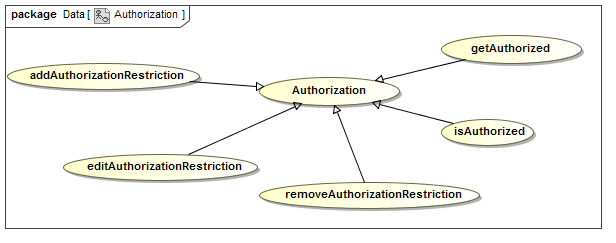
\includegraphics[width=1\linewidth]{./Graphics/Authorization}
Administration  users will be able to add, remove, and edit authorization restricitions. Authorization restrictions refer to the services that a user cannot access. If a certrain user group has a restiction on a service they will not be able to access that service. It can be assumed that if there is no restriction on a service then all users can access that service.


\subsection{addAuthorized}
\textbf{Description:}
This use case allows the administration user to add an authorization restriction on a user.
\subsubsection{Prioritization:}
Critical
\subsubsection{Conditions and Data Structures:}
\textbf{Pre-Conditions:}
\begin{itemize}
	\item User must have Administrator rights on  the system.
	\item Restriction must not exist.
\end{itemize}
\textbf{Post-Conditions:}
\begin{itemize}
	\item Restrictions must persist until removed
\end{itemize}
\subsubsection{Service Contract:}
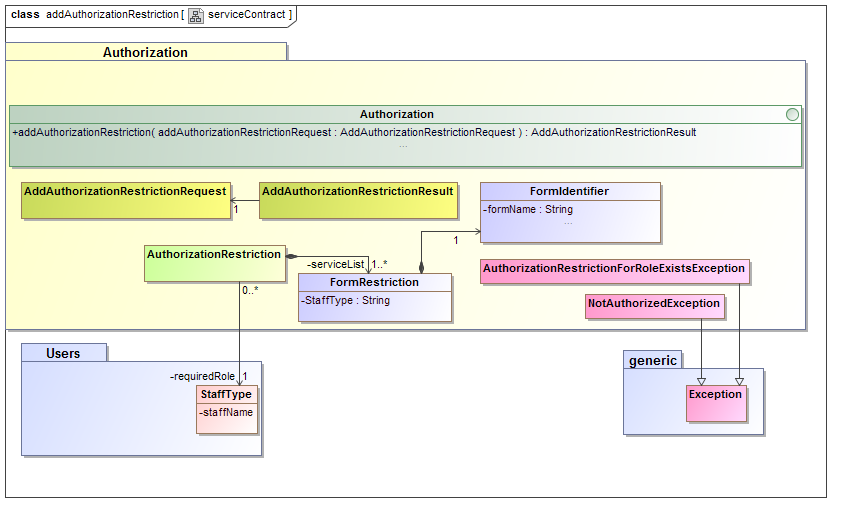
\includegraphics[width=1\linewidth]{./Graphics/addAuth}

\subsection{getAuthorised}
\textbf{Description:}
This use case allows an admin user to get all the authorization features.
\subsubsection{Prioritization:}
Important
\subsubsection{Conditions and Data Structures:}
\textbf{Pre-Conditions:}
\begin{itemize}
	\item User is an administrator.
\end{itemize}
\textbf{Post-Conditions:}
\begin{itemize}
	\item Results are returned to the administrator.
\end{itemize}
\subsubsection{Service Contract:}
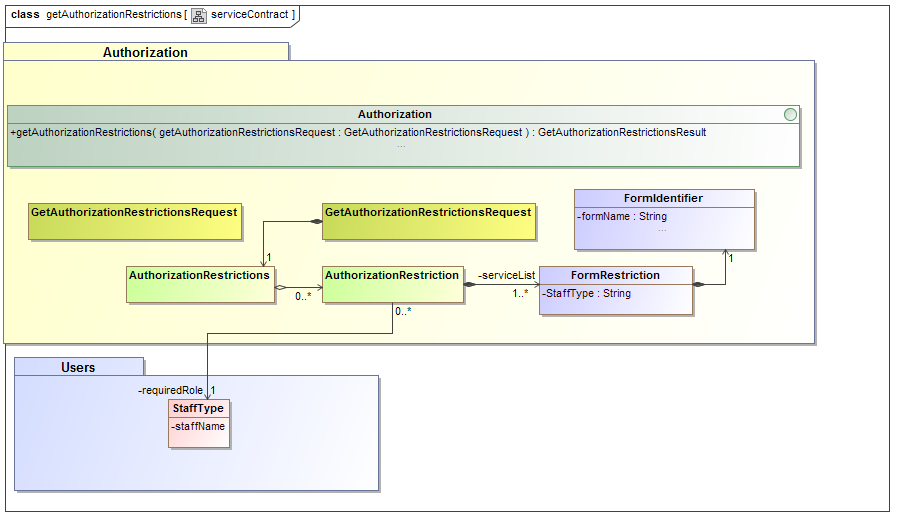
\includegraphics[width=1\linewidth]{./Graphics/getAuthorized}

\subsection{removeAuthorized}
\textbf{Description:}
This use case allows the administration user to remove an authorization restriction on a user.
\subsubsection{Prioritization:}
Critical
\subsubsection{Conditions and Data Structures:}
\textbf{Pre-Conditions:}
\begin{itemize}
	\item User has an administration role	
\end{itemize}
\textbf{Post-Conditions:}
\begin{itemize}
	\item Authorization restriction is removed from the data base
\end{itemize}
\subsubsection{Service Contract:}
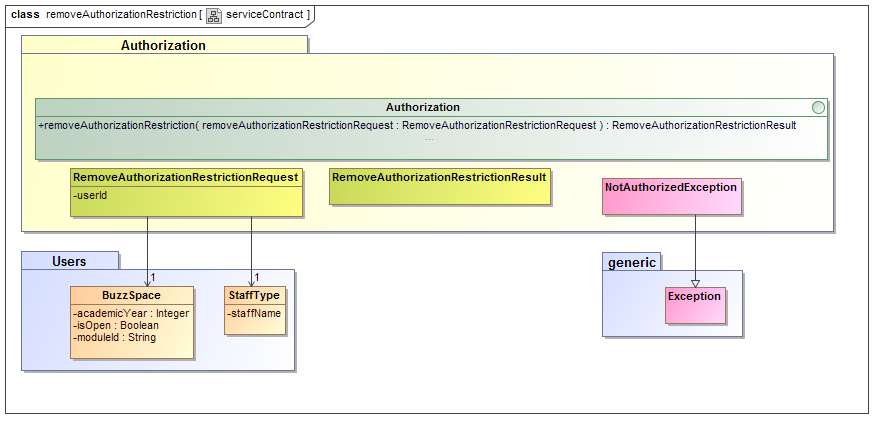
\includegraphics[width=1\linewidth]{./Graphics/RemoveAuth}

\subsection{editAuthorized}
\textbf{Description:}
This use case allows the administration user to edit authorization restrictions on users
\subsubsection{Prioritization:}
Important
\subsubsection{Conditions and Data Structures:}
\textbf{Pre-Conditions:}
\begin{itemize}
	\item User has an Administration Role
\end{itemize}
\textbf{Post-Conditions:}
\begin{itemize}
	\item Updated authorization restrictions are stored in database
\end{itemize}
\subsubsection{Service Contract:}
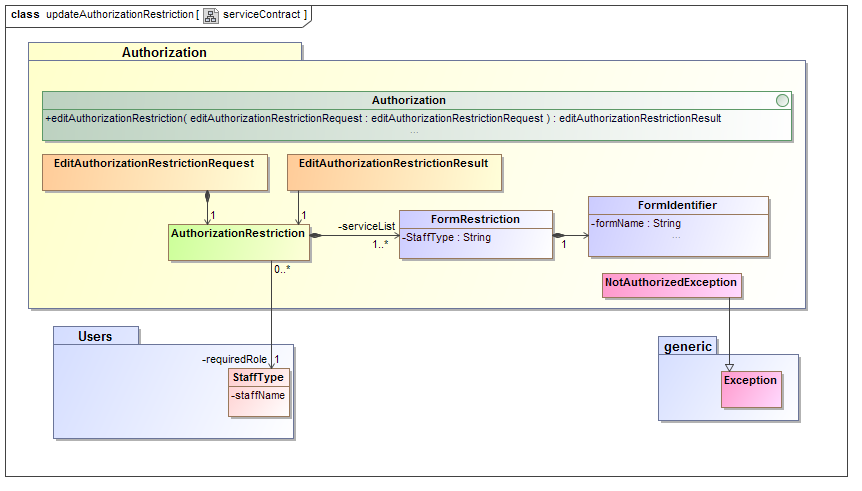
\includegraphics[width=1\linewidth]{./Graphics/updateAuth}


\subsection{isAuthorized}
\textbf{Description:}
This use case tests if a user is authorized to access a specific service
\subsubsection{Prioritization:}
critical
\subsubsection{Conditions and Data Structures:}
\textbf{Pre-Conditions:}
\begin{itemize}
	\item User is authorized to access service
\end{itemize}
\textbf{Post-Conditions:}
\begin{itemize}
	\item User is permitted to access the service.
\end{itemize}
\subsubsection{Service Contract:}
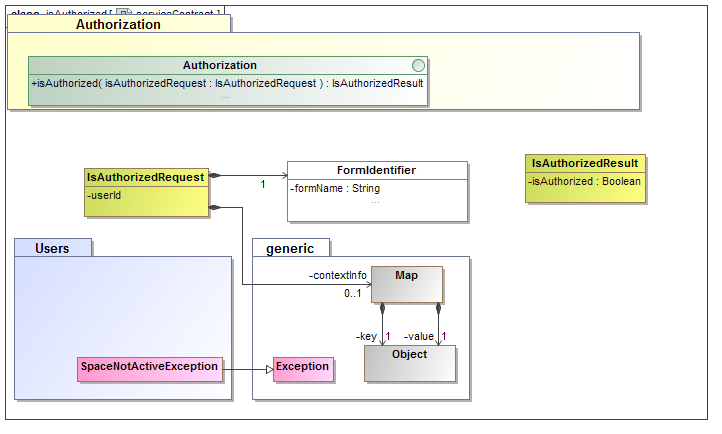
\includegraphics[width=1\linewidth]{./Graphics/isAuthorized}